\chapter{Grundlagen}
\label{chap:grundlagen}

In diesem Abschnitt meiner Arbeit, möchte ich zu erst die nötigen Grundlagen behandeln, um ein Basiswissen für die folgenden Kapitel sicherzustellen.\\
Da sich die Arbeit hauptsächlich um den Bildmerkmal Algorithmus \textbf{Histogram of Oriented Gradients} Algorithmus dreht, fange ich mit diesem an.
\section{Histogram of Oriented Gradients}
\label{sec:grundlagenhog}
Wie gerade erwähnt ist der \textbf{HOG} ein Bildmerkmal Algorithmus, der sich gegen bekannte Algorithmen (z.B. SIFT) bestens schlägt und dabei  effizienter arbeitet. Entwickelt und vorgestellt wurde der Algorithmus von Navneet Dalal und Bill Triggs im Paper \emph{Histograms of oriented Gradients for Human Detection} \cite{dalal:inria-00548512} veröffentlicht.\\
Grundlegend funktioniert der Algorithmus durch das Beschreiben von Verläufen. Diese Informationen werden in ein geeignetes Format gebracht um anschließend das betrachtete Bild zu klassifizieren. Wie in der ursprünglichen Arbeit, wird in dieser Arbeit erkannt ob ein Mensch in  einem Bild vorhanden ist. Der gesamten Ablauf ist in der Abbildung 2.1 dargestellt. \cite{dalal:inria-00548512}
\begin{figure}[htbp]\centering
	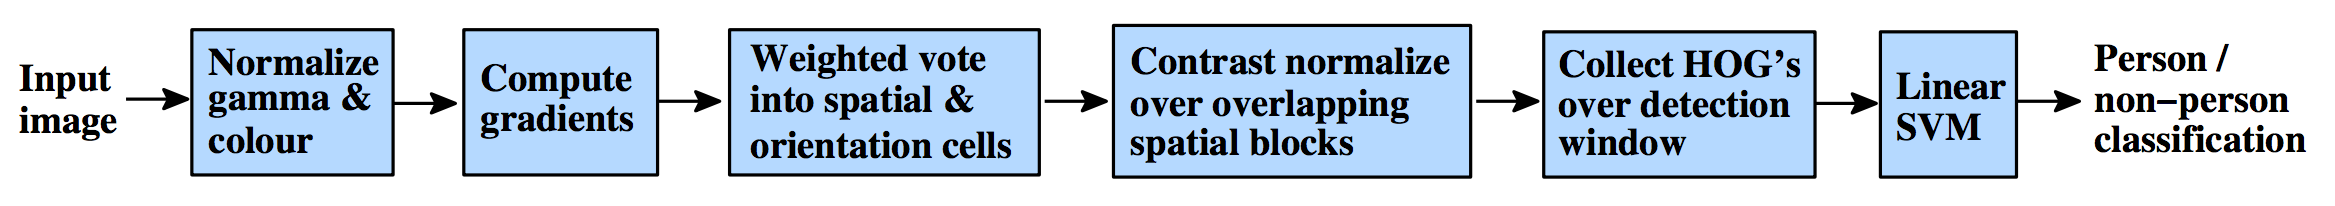
\includegraphics[width=1\linewidth]{./pics/featureextractionchain.png} 
	\caption{Ablauf der Klassifizierung von Bildmerkmalen}
	\label{fig:grundlagen_feature_extraction_chain}
\end{figure}

%    \begin{comment}
%    \begin{figure}
%    \begin{center}
%    \smartdiagramset{
%        circular distance=4cm,
%        font=\small,
%        text width=3.5cm,
%        module minimum width=3.8cm,
%        module minimum height=1.5cm,
%        arrow tip=to,
%        set color list={blue!50!cyan,green!60!lime,orange!50!red,red!80!black}
%    }
%    \smartdiagram[circular diagram]{Bild laden, Gradienten berechnen, Zellen-Histogramme erstellen, %Blöcke normalisieren, Feature-Vektor zusammenfassen, SVM-Klassifizierung}
%    \caption{Ablauf der Klassifizierung von Bildmerkmalen}
%    \label{fig:grundlagen_feature_extraction_chain}
%    \end{center}
%    \end{figure}
%    \end{comment}
Die wichtigsten Bestandteile werde ich im Folgenden erklären.

\subsection{Gradienten-Vektoren}

Wie der Name zu erkennen gibt, betrachtet der \textbf{HOG}-Algorithmus die Gradienten eines Bildes. Beschrieben werden Gradienten durch Vektoren:

$$
\vec{g}=\begin{pmatrix}
	g_x \\
	g_y
\end{pmatrix}
$$

Um die Elemente $g_x$ und $g_y$ zu berechnen, gibt es einige mögliche Filter. Laut \emph{Dalal} und \emph{Triggs} \cite[S.5]{dalal:inria-00548512} funktioniert der simple Filter


$$
\vec{x}=\begin{pmatrix}
	-1 & 0 & 1
\end{pmatrix}
$$
bzw.\\
$$
\vec{y}=\begin{pmatrix}
	-1 \\
	0 \\
	1
\end{pmatrix}
$$

am besten.
Diese Filter werden auf jeden Bildpunkt im Bild angewandt. Somit ergibt sich die Berechnung von $g_x$ und $g_y$ zu:
\begin{equation*}
	g_{x_k}=-x_{k-1}+x_{k+1} \\
	g_{y_k}=-y_{k-1}+y_{k+1}
\end{equation*}

Dabei ist $x_k$ der betrachtete horizontale Bildpunkt und $y_k$ ist der betrachtete vertikale Bildpunkt.\\
Jedoch aufgepasst, man muss beachten, dass bei einem Farbbild $g_x$ und $g_y$ für jeden Farbkanal berechnet werden müssen. Zusätzlich verhält sich die Berechnung am Rand des Bildes etwas anders.
Wie in der Abbildung 2.2 dargestellt, wird der Wert des Bildpunktes am Rand für die Berechnung einfach wiederholt.


\begin{figure}[h]
\centering

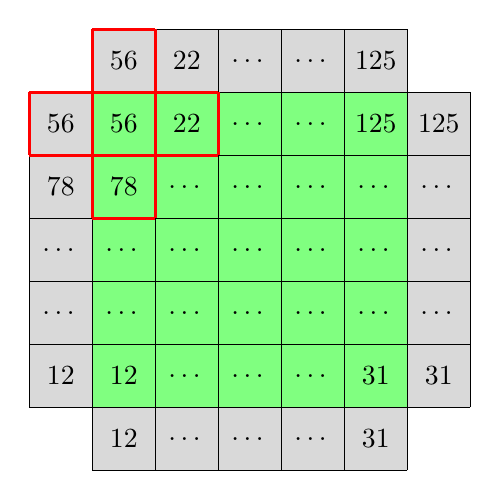
\begin{tikzpicture}[
        x=0.8 cm,
        y=0.8 cm]
        
%Hintergrund
\fill[green!50] (1,1) rectangle (6,6);
\fill[gray!30] (1,0) rectangle (6,1);
\fill[gray!30] (1,6) rectangle (6,7);
\fill[gray!30] (0,1) rectangle (1,6);
\fill[gray!30] (6,1) rectangle (7,6);
%Außenrand
\draw[] (1,0)--(6,0);
\draw[] (0,1)--(0,6);
\draw[] (7,1)--(7,6);
\draw[] (1,7)--(6,7);
%Vertikale Linien
\draw[] (1,0)--(1,7);
\draw[] (2,0)--(2,7);
\draw[] (3,0)--(3,7);
\draw[] (4,0)--(4,7);
\draw[] (5,0)--(5,7);
\draw[] (6,0)--(6,7);
%Horizontale Linien
\draw[] (0,1)--(7,1);
\draw[] (0,2)--(7,2);
\draw[] (0,3)--(7,3);
\draw[] (0,4)--(7,4);
\draw[] (0,5)--(7,5);
\draw[] (0,6)--(7,6);
%Markierter Bereich Horizontal
\draw[very thick,color=red] (1,4)--(1,7);
\draw[very thick,color=red] (2,4)--(2,7);
\draw[very thick,color=red] (1,7)--(2,7);
\draw[very thick,color=red] (1,4)--(2,4);
%Markierter Bereich Vertikal
\draw[very thick,color=red] (0,6)--(3,6);
\draw[very thick,color=red] (0,5)--(3,5);
\draw[very thick,color=red] (0,6)--(0,5);
\draw[very thick,color=red] (3,6)--(3,5);
%Werte In Der Tabelle
\node[] at (0.5,5.5) {56};
\node[] at (1.5,5.5) {56};
\node[] at (1.5,6.5) {56};

\node[] at (6.5,5.5) {125};
\node[] at (5.5,5.5) {125};
\node[] at (5.5,6.5) {125};

\node[] at (2.5,5.5) {22};
\node[] at (2.5,6.5) {22};

\node[] at (0.5,4.5) {78};
\node[] at (1.5,4.5) {78};

\node[] at (1.5,1.5) {12};
\node[] at (0.5,1.5) {12};
\node[] at (1.5,0.5) {12};

\node[] at (5.5,1.5) {31};
\node[] at (5.5,0.5) {31};
\node[] at (6.5,1.5) {31};
%Punkte Für Die Unwichtigen Werte
\node[] at (2.5,0.5) {\dots};
\node[] at (3.5,0.5) {\dots};
\node[] at (4.5,0.5) {\dots};

\node[] at (2.5,1.5) {\dots};
\node[] at (3.5,1.5) {\dots};
\node[] at (4.5,1.5) {\dots};

\node[] at (0.5,2.5) {\dots};
\node[] at (1.5,2.5) {\dots};
\node[] at (2.5,2.5) {\dots};
\node[] at (3.5,2.5) {\dots};
\node[] at (4.5,2.5) {\dots};
\node[] at (5.5,2.5) {\dots};
\node[] at (6.5,2.5) {\dots};

\node[] at (0.5,3.5) {\dots};
\node[] at (1.5,3.5) {\dots};
\node[] at (2.5,3.5) {\dots};
\node[] at (3.5,3.5) {\dots};
\node[] at (4.5,3.5) {\dots};
\node[] at (5.5,3.5) {\dots};
\node[] at (6.5,3.5) {\dots};

\node[] at (2.5,4.5) {\dots};
\node[] at (3.5,4.5) {\dots};
\node[] at (4.5,4.5) {\dots};
\node[] at (5.5,4.5) {\dots};
\node[] at (6.5,4.5) {\dots};

\node[] at (3.5,5.5) {\dots};
\node[] at (4.5,5.5) {\dots};

\node[] at (3.5,6.5) {\dots};
\node[] at (4.5,6.5) {\dots};

\end{tikzpicture}

\caption{Randverhalten bei der Gradienten-Berechnung}
\label{fig:hog_randverhalten}
\end{figure}

Um nun Histogramme zu erstellen benötigt man für den HOG-Algorithmus zwei Werte. Einmal die Magnitude des Gradienten und dessen Orientierung.\\
Die Magnitude wird nach dem Satz von Pythagoras durch:
$$\lvert G \rvert = \sqrt{\strut{g_{x_k}^{2}+g_{y_k}^{2}}}$$
berechnet und die Orientierung durch:
$$ \theta=\arctan\frac{g_{x_k}}{g_{y_k}}. $$

\subsection{Histogramm-Erzeugung}

Dalal und Triggs Untersuchungen haben ergeben, dass Histogramme, welche eine Zelle von $8\times8$ Pixeln beschreiben, mit 9 Klassen (\emph{bins}) das beste Verhältnis von Genauigkeit zu Performanz hervorbringen.\\
Ein solches Histogramm entsteht durch gewichtetes \emph{binning} (die Gruppierung zu Klassen) der Magnitude und der dazu gehörigen Orientierung.
Die \emph{bins}-Intervalle entstehen, für die vorzeichenlosen Variante, durch die Aufteilung von 180$^\circ$ auf die gewünschte Anzahl von bins.
Beispielsweise würden die \emph{bins} wie folgt aussehen, wenn man nach Dalal und Triggs geht und 9 \emph{bins} benutzt: 
[$10^\circ,30^\circ,50^\circ,70^\circ,90^\circ,110^\circ,130^\circ,150^\circ,170^\circ$].\\
Würde man nun ein Magnituden-Wert von $16$ mit einer Orientierung von $85^\circ$ in ein solches Histogramm eintragen wollen, ist das gewichtete Resultat die Addition von einem Viertel der Magnitude auf den 4. \emph{bin} ($70^\circ$) und drei Viertel auf den 5. \emph{bin} ($90^\circ$).

\vspace*{5 mm}
! EIN HISTOGRAMM !
\vspace*{5 mm}

Daraus ergibt sich, wenn auf ein gesamtes Bild angewandt, ein Vektor von Histogrammen. Die Anzahl dieser Histogramme im Vektor, ergibt sich durch die Größe des Betrachteten Bildes und der gewählten Zellen-Größe.\\
und kommen schlussendlich zum letzten Schritt der Bildmerkmal-Erzeugung, dem Normalisieren.

\subsection{Block-Normalisierung}

In der Praxis kann man nicht garantieren, dass dem Algorithmus ein perfekt geschossenes Bild eingespeist wird. Das Bild kann z.B. durch schlechte Lichtquellen zu dunkel, zu hell sein oder sogar stellenweise Unterschiede aufweisen, was zur Normalisierung des betrachteten Bildes führt.

\vspace{5 mm}
! BEISPIEL BILD MIT ZELLEN UND BLÖCKEN !
\vspace{5 mm}

Laut der Arbeit von Dalal und Triggs, erhält man sehr gute Ergebnisse mit der Normalisierung von Blöcken, welche aus mehreren Zellen bestehen. Des weiteren resultierte die beste Erkennungsrate aus der Normalisierung von einem Block, der aus vier Zellen und somit aus vier Histogrammen bestand, was einen Bereich von 8 $\times$ 8 Pixel $\times$ 4 Zellen = 256 Pixel aufspannt.
Folglich entsteht ein \emph{Feature-Vektor} welcher die Bildmerkmale des gesamten Bildes beschreibt.\\
Die Normalisierung selbst erfolgt durch mathematische Funktionen, welche auf die Block-Histogramme angewandt werden. Bezüglich der Erkennungsrate ergeben die folgenden Normen ein ähnliches Ergebnis:

$$\mathrm{L1-sqrt:\ } f=\sqrt{\frac{v}{\lvert\lvert v \rvert\rvert_1+e}}$$
\vspace{5 mm}
$$\mathrm{L2-Norm:\ } f=\frac{v}{\sqrt{\strut{\lvert\lvert v \rvert\rvert^2_2+e^{2}}}}$$

Und \emph{L2-Hys}, bei der die L2-Norm angewandt wird und die Werte in v auf 0.2 begrenzt und anschließend erneut mit der L2-Norm normalisiert werden. Dabei sei $v$ der unnormierte Vektor, bestehend aus den Histogrammen der betrachteten Block-Zellen und $e$, einer Konstante mit einem geringen Wert, die das Ergebnis nicht beeinflusst.\\
Zusätzlich haben Untersuchungen ergeben, dass bei der Normalisierung eine Überlappung der Blöcke von 50\% die Erkennungsrate merkbar steigert. Dabei wird bei der Normalisierung eines Blockes, die rechte Hälfte des vorherigen, bereits normalisierten Blockes miteinbezogen. \cite{dalal:inria-00548512}
\begin{figure}[htbp]\centering 
	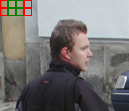
\includegraphics[width=.4\linewidth,resolution=90]{./pics/BlockBildHOG.png} 
	\caption{Eine Visualisierung der Überlappung von Blöcken}
	\label{fig:hog_overlap_example}
\end{figure}\\
Der Feature-Vektor beinhaltet schließlich für ein 64 $\times$ 128 Pixel großes Bild und einer Zellen-Größe von 8 $\times$ 8 Pixel bei 9 bins insgesamt 1152 Werte. Um ein Bild zu klassifizieren, wird der dazugehörige Feature-Vektor einer angelernten \emph{Support Vector Machine} übergeben, die ein positives oder negatives Ergebnis hervorbringt und somit bestimmt ob ein Mensch auf dem Bild erkannt wird oder nicht.

\section{Support Vector Machine}
\label{sec:grundlagensvm}

Die \emph{Support Vector Machine} ist ein Modell des maschinellen Lernens, mit dem Mengen-Elemente klassifiziert werden können. Dies kann für linear-trennbare Mengen geschehen oder aber auch für nicht-lineare. Im folgenden wird nur das Verfahren der linearen Trennung vorgestellt, da dies für das Verständnis dieser Arbeit genügt.

\subsection{Prinzip}

Die grundlegende Funktion der SVM besteht darin Eingabe-Daten zu verarbeiten und anschließend zu bestimmen zu welcher Klasse sie gehören. Eine Beispiel-Menge die klassifiziert werden soll ist anhand Abbildung 2.3 dargestellt. Wie man sieht könnte man einfach einige Geraden ziehen, die beide Klassen trennen. Die Überlegung ist nun wie man die beste Gerade (zweidimensionale Hyperebene) findet.

\begin{figure}[h!]
\begin{subfigure}[b]{0.45\textwidth}
\centering
\begin{tikzpicture}[
        x=0.9 cm,
        y=0.9 cm]
\draw[->, thick, draw=black] (0,0)--(5,0) node (xaxis) [right] {$X_1$};
\draw[->, thick, draw=black] (0,0)--(0,5) node (yaxis) [above] {$X_2$};
\foreach \Point in {(3,3.5), (1,2), (2,4), (2,3.5), (2,4),(1,3.5)}{
    \fill[black] \Point circle(2pt);
}
\foreach \Point in {(4.5,2), (1.5,1), (3,2), (2.5,1), (3,1),(2,0.5)}{
    \fill[black] \Point circle(2pt);
}
\end{tikzpicture}
\end{subfigure}
\begin{subfigure}[b]{0.45\textwidth}
\begin{tikzpicture}[
        x=0.9 cm,
        y=0.9 cm]
\draw[dashed,thin,draw=blue!80] (0,0)--(4.4,4.4);
\draw[dashed,thin,draw=blue!80] (0,0.5)--(4.5,4.0);
\draw[dashed,thin,draw=blue!80] (0,1)--(4.5,3.6);
\draw[->, thick, draw=black] (0,0)--(5,0) node (xaxis) [right] {$X_1$};
\draw[->, thick, draw=black] (0,0)--(0,5) node (yaxis) [above] {$X_2$};
\foreach \Point in {(3,3.5), (1,2), (2,4), (2,3.5), (2,4),(1,3.5)}{
    \node [green] at \Point {$\boldsymbol{+}$};
}
\foreach \Point in {(4.5,2), (1.5,1), (3,2), (2.5,1), (3,1),(2,0.5)}{
    \node [red] at \Point {$\boldsymbol{-}$};
}
\end{tikzpicture}
\end{subfigure}
\caption{Ausgangs Vektoren-Menge}
\label{fig:svm_coordinate_system_start}
\end{figure}

\subsection{Klassifizierung}

Allgemein ist die Funktion der Klassifizierung definiert durch $f:X\subseteq\mathbb{R}^n\to\mathbb{R}$, welche einen Vektor $\vec{x}$ als Eingabe bekommt und diesen auf einen reellen Wert abbildet. Eine Eingabe wird \emph{positiv} klassifiziert falls $f(x) \ge 0$ gilt, ansonsten wird sie der Klasse \emph{negativ} zugeordnet. \cite{cristianini2000introduction}\\
Geometrisch betrachtet ergibt sich eine Hyperebene, welche durch die Funktion $f(x)=\langle\vec{w}\cdot\vec{x}\rangle+b$ beschrieben wird, wobei $\vec{w}$ den Richtungsvektor darstellt, der senkrecht auf der Hyperebene steht und $b$ die Verschiebung parallel zur Hyperebene beschreibt, auch \emph{bias} genannt.\\
Es ist nun bekannt, dass ein $\vec{x}$ mit $\langle\vec{w}\cdot\vec{x}\rangle+b\ge0$ der positiven Klasse und mit $\langle\vec{w}\cdot\vec{x}\rangle+b<0$ der negativen Klasse zugeordnet wird. Um nun eine Hyperebene aufzuspannen die beide Klassen zuverlässig trennt müssen $\vec{w}$ und $b$ gut gewählt werden.\\
Dazu werden Trainingsobjekte benötigt, von denen man weiß zu welcher Klasse sie gehören. Durch die Nutzung solcher Trainingsobjekte gehört der Trainingsvorgang der SVM zum \emph{Überwachten Lernen}. Die Namensgebung verrät schon, dass im Training mithilfe der Informationen eine Selbstkontrolle erfolgt, die eine berechnete Parameter-Kombination entweder bestätigt oder verwirft.\\
Vorher muss aber noch ein Problem gelöst werden.

\begin{figure}[h!]
\centering

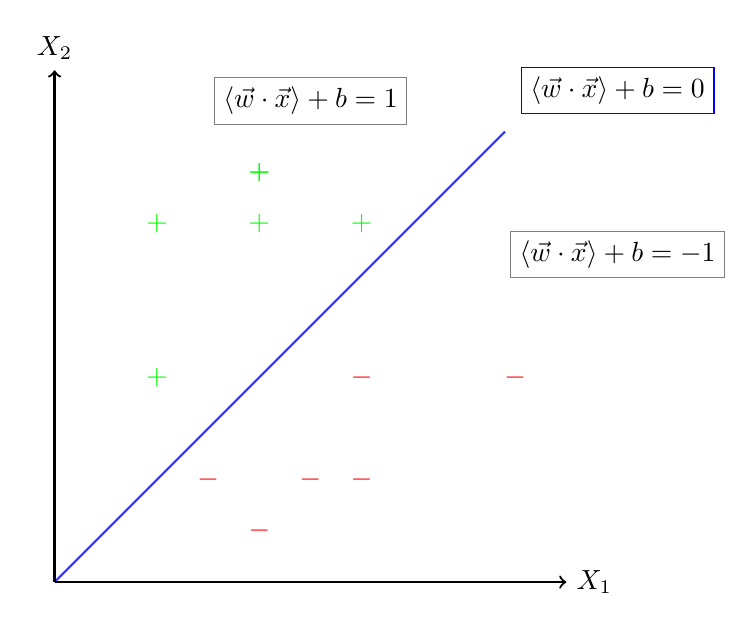
\begin{tikzpicture}[
        x=1.3 cm,
        y=1.3 cm]
  
\draw[thick, draw=blue!80] (0,0)--(4.4,4.4);
\draw[->, thick, draw=black] (0,0)--(5,0) node (xaxis) [right] {$X_1$};
\draw[->, thick, draw=black] (0,0)--(0,5) node (yaxis) [above] {$X_2$};

\tkzDefPoints{0/0/S,4.4/4.4/E,3/3.5/SPOS,1.5/1/SNEG,-.25/-.25/LPOS,.25/.25/LNEG,-.25/.25/LEFT,1.15/1.15/LEFTTOP, .25/-.25/RIGHT,3.2/3.2/RIGHTTOP}
\tkzDefLine[orthogonal=through SPOS](S,LPOS) \tkzGetPoint{c}
\tkzDrawLine[add=0 and 0,style=dashed,thick](SPOS,c)

\tkzDefLine[orthogonal=through SNEG](S,LNEG) \tkzGetPoint{d}
\tkzDrawLine[add=0 and 0,style=dashed,thick](SNEG,d)

\tkzDefLine[parallel=through SPOS](S,LEFTTOP) \tkzGetPoint{e}
\tkzDrawLine[add=0 and 0,style=dashed,color=gray,very thin](LEFT,e)

\tkzDefLine[parallel=through SNEG](S,RIGHTTOP) \tkzGetPoint{f}
\tkzDrawLine[add=0 and 0,style=dashed,color=gray,very thin](RIGHT,f)


\foreach \Point in {(3,3.5), (1,2), (2,4), (2,3.5), (2,4),(1,3.5)}{
    \node [green] at \Point {$\boldsymbol{+}$};
}
\foreach \Point in {(4.5,2), (1.5,1), (3,2), (2.5,1), (3,1),(2,0.5)}{
    \node [red] at \Point {$\boldsymbol{-}$};
}

\node[draw=blue] at (5.5,4.8) {$\langle\vec{w}\cdot\vec{x}\rangle+b=0$};
\node[draw=gray] at (2.5,4.7) {$\langle\vec{w}\cdot\vec{x}\rangle+b=1$};
\node[draw=gray] at (5.5,3.2) {$\langle\vec{w}\cdot\vec{x}\rangle+b=-1$};
\end{tikzpicture}
\caption{Klassifizierung durch \emph{Stütz}-Vektoren}
\label{fig:svm_coordinate_system}
\end{figure}

Da die Hyperebene durch $h(x)=\langle\vec{w}\cdot\vec{x}\rangle+b=0$ beschrieben ist macht es keinen Unterschied welche Werte $\vec{w}$ und $b$ annehmen, da für ein beliebiges $c\neq 0$ $(cw,cb)$ das selbe Ergebnis wie für $(w,b)$ resultiert. Folglich wird das Paar $(w,b)$ relativ zu den Trainingsobjekten skaliert, so dass $min\lvert\langle w,x_i \rangle +b\rvert=1$ gilt.\\
Als nächstes ist der größte trennende Bereich der zwei Klassen zu finden. Dazu betrachtet man den Abstand $d(x_i,h(x))$, wobei $x_i$ der Klasse $y_i\in\{+1,-1\}$ zugehört und $h(x)$ die Hyperebenenfunktion: $\langle w,x \rangle+b=0$ ist. Dieser Abstand lässt sich berechnen mit:
$$ d(h(x),x_i)=y_i(\langle\frac{w}{\lvert\lvert w \rvert\rvert},x_i\rangle + \frac{b}{\lvert\lvert w \rvert\rvert)}$$
Dank der vorherigen Skalierung ergibt sich für die beiden Traininsgobjekte $(x_1,+1)$ und $(x_2,-1)$ folgende Rechung:
\begin{align*}
    \langle w,x_1 \rangle+b=+1
    & \Rightarrow%\text{ und }
    \langle \frac{w}{\lvert\lvert w \rvert\rvert},x_1\rangle+\frac{b}{\lvert\lvert w \rvert\rvert}=\frac{1}{\lvert\lvert w \rvert\rvert}\notag\\
    \langle w,x_2 \rangle+b=-1
    & \Rightarrow%\text{ und }
    \langle \frac{w}{\lvert\lvert w \rvert\rvert},x_2\rangle+\frac{b}{\lvert\lvert w \rvert\rvert}=\frac{-1}{\lvert\lvert w \rvert\rvert}\notag\\
    & \Rightarrow \langle \frac{w}{\lvert\lvert w \rvert\rvert},(x_1-x_2)\rangle=\frac{2}{\lvert\lvert w \rvert\rvert}\notag
\end{align*}

mit der das Resultat $\frac{2}{\lvert\lvert w \rvert\rvert}$ die Trennspanne zwischen der positiven und negativen Klasse beschreibt. Um nun die maximale Trennspanne zu erreichen muss, wie man sehen kann, $\lvert\lvert w \rvert\rvert$ minimiert werden. Zusätzlich muss die Bedingung $y_i(\langle w,x_i \rangle + b \geq 1$ für $i=1,\dots,n$ eingahalten werden, um sicherzustellen, dass die Trainingsobjekte anhande der Hyperebene der richtigen Klasse zugewiesen werden.\\
Es liegt nun ein Optimierungsproblem vor, welches mithilfe der Lagrange-Funktion $L(w,b,a)$ beschrieben werden kann:
\begin{align}
L(w,b,a) = \frac{1}{2}\lvert\lvert w \rvert\rvert^2-\sum\limits_{i=1}^n a_i(y_i(\langle w,x_i \rangle + b)-1)\notag
\end{align}

Diese Funktion wird für $(w,b)$ minimiert und für $a_i$ maximiert. Man erhält durch:
\begin{align}
\frac{d}{db}L(w,b,a)=0 \text{ und } \frac{d}{dw}L(w,b,a)=0\notag
\end{align}
das Ergebnis:
\begin{align}
\sum\limits_{i=1}^n a_i y_i=0\text{ und } w=\sum\limits_{i=1}^n a_i y_i x_i\notag
\end{align}

Dieses Ergebnis wiederum kann wieder in die $L(a,b,a)$ eingesetzt werden und man erhält umgeformt das duale Problem der Maximierung von:
\begin{align}
W(a)=\sum\limits_{i=1}^n a_i - \frac{1}{2}\sum\limits_{i=1}^n a_i a_j y_i y_j \langle x_i,x_j \rangle\notag
\end{align}
mit den Bedingungen:
\begin{align}
a_i \geq 0 \text{ und } \sum\limits_{i=1}^n a_i y_i =0\notag
\end{align}
Durch das lösen des dualen Problems erhält man die $a_i$, welche $W(a)$ maximieren. Mit diesen ist es nun möglich den Normalvektor $w$ mit $w=\sum a_i y_i x_i$ zu bestimmen, mit dem die trennende Hyperebene beschrieben werden kann, welche die maximale Trennspanne besitzt. Die gesuchte Entscheidungsfunktion ergibt sich schließlich zu:
\begin{align}
f(x_{neu})&=sign(\langle w,x_{neu} \rangle + b)\\
&=sign(\sum\limits_{i=1}^n a_i y_i \langle x_i,x_{neu} \rangle +b)
\end{align}

7. Warum Support Vektoren\\
8. Perzeptron Algorithmus\\


Die Parameter $\vec{w}$ und $b$ werden durch durch das \emph{Antrainieren} der SVM festgelegt, welches im nächsten Abschnitt erklärt wird.

\subsection{Überwachtes Lernen}





$\langle\vec{w}\cdot\vec{x}\rangle+b=0$









\section{Tensilica Xtensa LX5}
\label{sec:grundlagenlx5}

\section{Tensilica Instruction Extension}
\label{sec:grundlagentie}

\section{Assembler}
\label{sec:grundlagenassembler}